
\begin{frame}
	\frametitle{Problem definition and analytical solution}
	\begin{itemize}
		\item 1D HC with T = 0 at boundaries and heat source, Q = 2.0
			\vspace{1cm}
		\item Analytical solution obtained using the method of manufactured solutions
			\begin{align*}
				T(x) = x - x^2
			\end{align*}

		\item Governining equation

			\begin{align*}
				K\frac{d^2 T}{d x^2} + Q = 0
			\end{align*}
	\end{itemize}
\end{frame}

%------------------------------------------------------------------------------


\begin{frame}
	\frametitle{Finite element fomulation}
	\begin{itemize}
		\item Galerkin method with linear shape function elements were used

			\begin{align*}
				\int_{0}^{L} \phi(x) \left(K\frac{d^2 T}{d x^2} + Q  \right) dx = 0
			\end{align*}

		\item Shape functions

			\begin{align*}
				N_1 &= 1 - \frac{x}{h} \\
				N_2 &= \frac{x}{h} && \text{h - spatial step size}
			\end{align*}

		\item Matrix equation
			\begin{align*}
				\frac{K}{h} \begin{bmatrix} 1 & -1 \\ -1 & 1 \end{bmatrix} \begin{bmatrix} T_1 \\ T_2 \end{bmatrix} = \frac{Q h}{2} \begin{bmatrix} 1 \\ 1 \end{bmatrix} + \begin{bmatrix} q_1 \\ q_2 \end{bmatrix}
			\end{align*}

	\end{itemize}
\end{frame}

%------------------------------------------------------------------------------

\begin{frame}
	\frametitle{Results - with 5 elements}
	Computed result
	\begin{figure}
		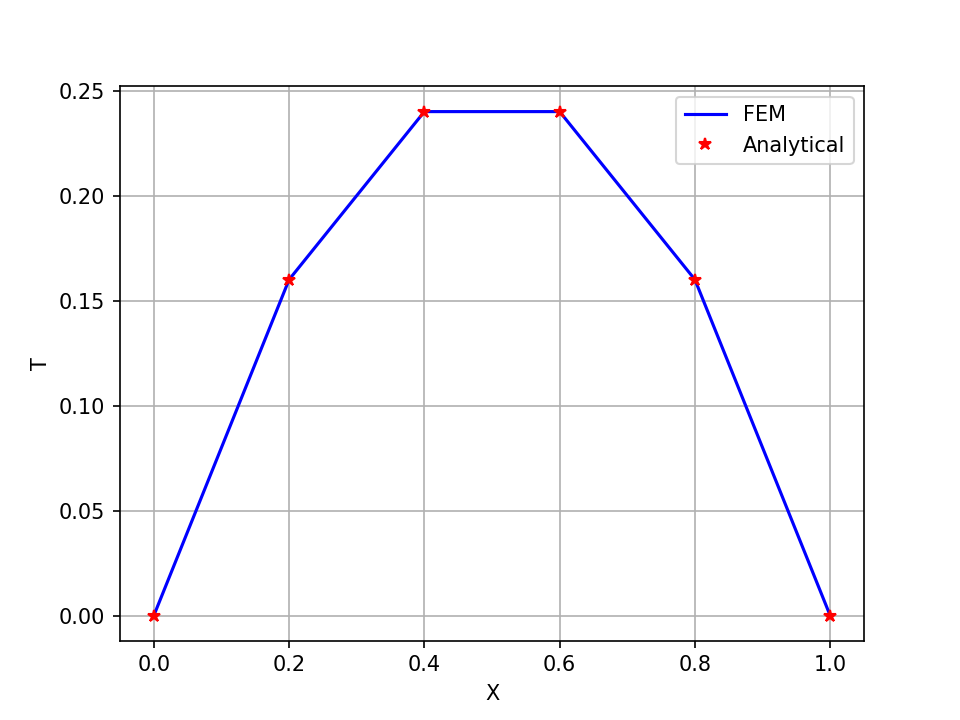
\includegraphics[scale=0.5]{supportingFiles/output_5.png}
	\end{figure}
\end{frame}

\begin{frame}
	\frametitle{Results - with 5 elements}
	Computed error
	\begin{figure}
		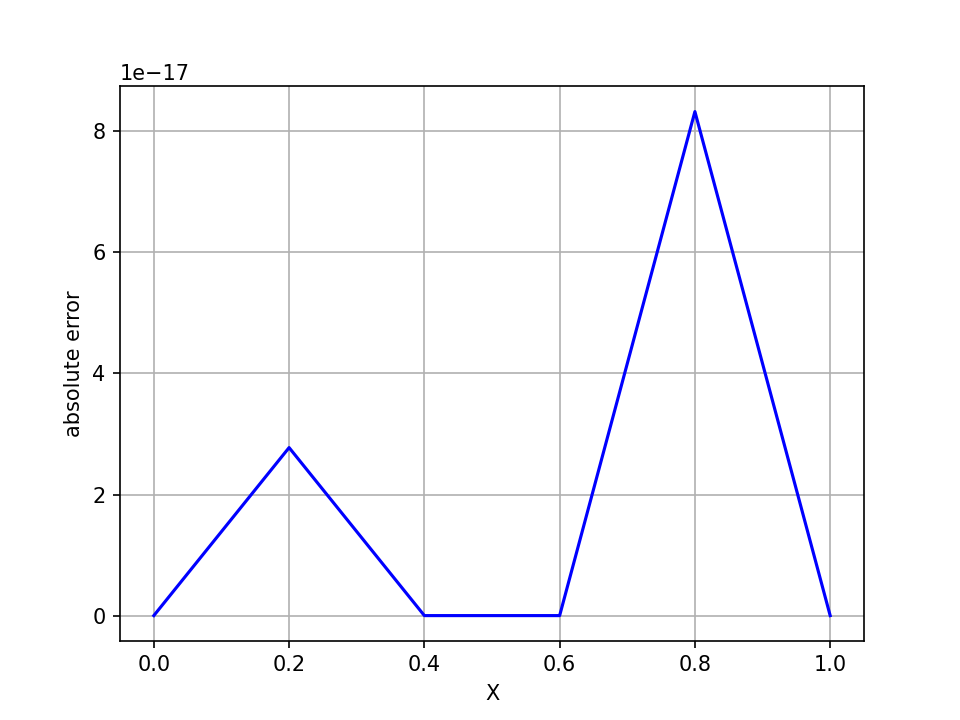
\includegraphics[scale=0.5]{supportingFiles/error_5.png}
	\end{figure}
\end{frame}

\begin{frame}
	\frametitle{Results - with 10 elements}
	Computed result
	\begin{figure}
		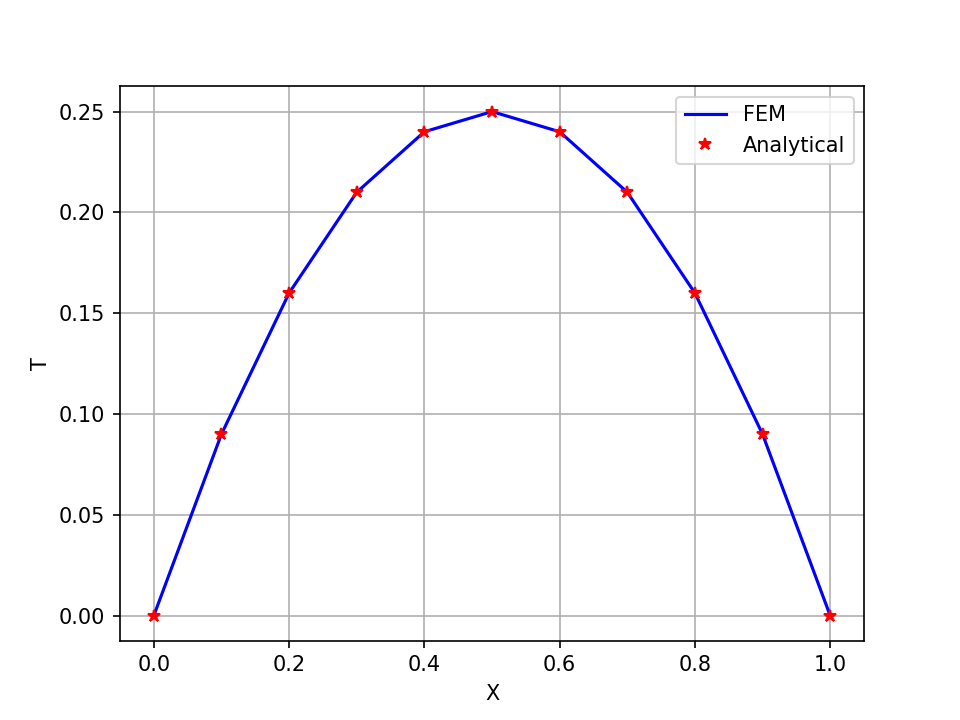
\includegraphics[scale=0.5]{supportingFiles/output_10.png}
	\end{figure}
\end{frame}

\begin{frame}
	\frametitle{Results - with 10 elements}
	Computed error
	\begin{figure}
		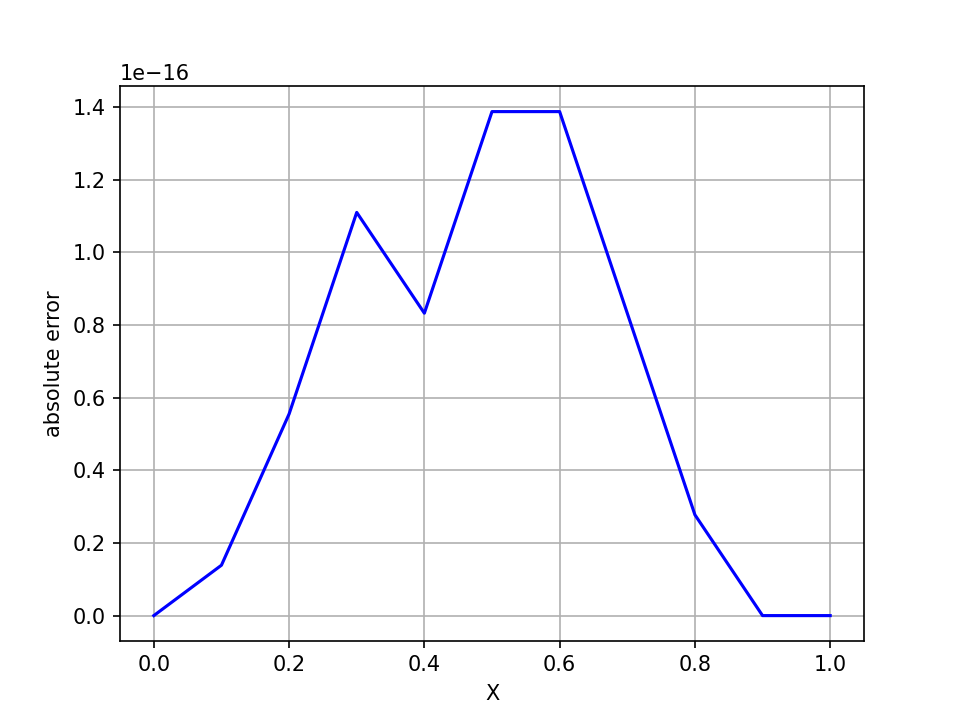
\includegraphics[scale=0.5]{supportingFiles/error_10.png}
	\end{figure}
\end{frame}

%------------------------------------------------------------------------------

\begin{frame}
	\frametitle{Reference}
Pepper, Darrell W., and Juan C. Heinrich. The finite element method: basic concepts and applications. Taylor \& Francis, 2005.
\end{frame}
